\chapter{Konzolová časť aplikácie na správu mikrotikov}
V tejto kapitole si popíšeme fungovanie naprogramovanej aplikácie. Celkovo je konzolová časť aplikácie napísaná za pomoci knižnice tikapy popísanej v kapitole \ref{sec:tikapy}. Kapitola bude rozdelená do niekoľkých častí:\begin{itemize}
\item časť 1: popis naprogramovanej časti pre vyhľadávanie mikrotikov, pripojenie sa na mikrotik cez python pomocou protokolov telnet, SSH, mactelnet a napojenie na metódy
\item časť 2: Popis infraštruktúry backendu - zložky, ich vysvetlenie, zoznam súborov na konfiguráciu mikrotku, vysvetenie rozdelenia, vysvetlenie tried, metód daných tried a volanie funkcií
\item časť 3 - prtidanie tabuliek jednotlivých tried a ich metód v každej zložke, krátka sumarizácia, ich niektoré vybrané UML diagramy, ostatné budú zahrnuté v prílohe
\end{itemize}
\section{Popis naprogramovanej časti prihlasovania na mikrotik}
\label{sec:popis1}
V tejto časti si zobrazíme rozbor časti prihlasovania na mikrotik a základné funnkcie. Toto je riadené v rámci projektu nazvaného \textit{diplomkap3} v ktorom je súbor \textit{loginManager.py}. V rámci login managera tu nachádzame:
\section{Rozbor hlavnej časti backendu}
V rámci hlavnej konfiguračnej časti diplomovej práce, pre konfiguráciu backendu mikrotiku za pomoci porgramovacieho jazyka python som projekt rozdelil do niekoľkých častí:\begin{itemize}
\item \textbf{bridge} - táto časť obsahuje prvky konfiguácie, pridania, odstránenia, zapnutia, vypnutia možnosti bridgu na mikrotiku, konfigurácia existujúceho bridgu, zobrazenie zoznamu bridgov
\item  \textbf{capsman} - táto časť obsahuje konfiguráciu hromadnej obsluhy mikrotik úrístupových bodov a WiFi, profily, bezpečnosť, konfiguácie, povolené rýchlosti, zobrazenie zoznamu pripojených prvkov a ďalšie funkcie
\item \textbf{certs} - obsahuje certifikáty na pripojenie sa na mikrotik pomocou protokolu api-ssl
\item \textbf{Dude} - obsahuje popis konfigurácie ako nastaviť nástroj Dude klienta, ako nakonfigurovať Dude na vzdialený monitoring na Dude serveri, taktiež Dude server, a ďalšie možnosti
\item \textbf{exportToHtml} - časť predstavuje generovanie súboru na analýzu v podobe webovej stránky
\item \textbf{interfaces} - časť predstavuje konfiguráciu rozhraní na mikrotiku, tieto časti sú tiež popísané aj v iných zložkách ako napr. bridge. 4asť popisuje pridanie, odstránenie, zapnutie, vypnutie, konfiguráciu existujúcich rozhraní.
\item \textbf{IPv4} - rozsiahla časť, obsahuje konfiguráciu IP adries, firewallu, monitoringu, smerovania a ďalších nástrojov spadajúcich pod IP zložku na mikrotiku.
\item \textbf{IPv6} - pre zložku IPv6 platí to isté čo pre zložku IPv4, ale platí pre konfiguráciu na základe IPv6 adresného rozsahu
\item \textbf{KVM} - sekcia bude popisovať možnosti virtualizácie mikrotiku.
\item \textbf{log} - sekcia bude popisovať analýzu a konfiguráciu logu zariadenia
\item \textbf{makeSupportFile} - seckia bude popisovať vytvorenie súboru potrebného pre analýzu na mikrotik podpore
\item \textbf{mesh} - sekcia popisuje konfiguráciu tzv. mesh technológie, technológii podobne ako  v rámci časti bridge
\item \textbf{MPLS} - sekcia bude popisovať možnosti konfiurácie Multi Protocol Label Switching (MPLS), jej pridanie, odstránenie ,zapnutie, vypnutie, modifikácie a ďalšie funkcie.
\item \textbf{PPP} - sekcia bude popisovať konfiguráciu Point to Point Protocol (PPP) a ďalších možností Virtual Private Network (VPN) konfigurácie.
\item \textbf{Queues} - sekcia budep popisovať konfiguráciu sieťových front, možnosti front, typy front a ďalšie funkcie
\item \textbf{Radius} - sekcia bude popisovať nastavenie funkcie Radius - autentizačnej služby užívateľov , jeho modifikáciu, konfiguráciu a ďalšie funkcie.
\item \textbf{Routing} - sekcia bude popisovať možnosti dynamického smerovania, statické smerovanie bude popísané v rámci časti IPv4, dynamické smerovacie protokoly, ich konfigurácie, a ďalšie možnosti. 
\item \textbf{Switch} - sekcia bude popisovať konfiguráciu prepínača, niektoré mikrotiky sú typu SwitchOS a sú štandardne prepínač. Kofiguuráciu portov, trunkov, a ďalších funkcií. 
\item \textbf{System} - sekcia bude popisovať časť konfigurácie systémových nástrojov, ich funkcií a konfigurácie, a ďalších funkcií.
\item \textbf{Tools} - sekcia bude popisovať konfiguráciu mikrotik nástroj, a však nie všetky bolo možné odsimulovať v rámci konzolvej časti aplikácie, ich konfiguráciu, spustenie, riadenie a ďalšie funkcie. 
\item \textbf{Wireless} - sekcia bude obsahovať konfiguráciu bezdrátového rozhrania, moduly, módy, konfiguráciu, nastavenie, a ďalšie funkcie
\item \textbf{konfiguračné súbory mimo zložiek} - sekcia popísaná v kapitole  \ref{sec:popis1}, popisuje súbory na základnú konfiuráciu mikrotiku, nastavenie základnej konfigurácie.
\end{itemize}
Ukážka súborovej štruktúry je zobrazená na obrázku \ref{fig:structure}:
\begin{figure}[H]
\centering
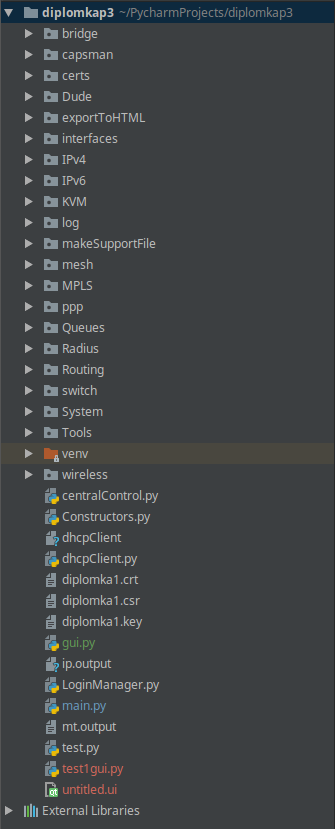
\includegraphics[scale=0.4]{../text/struktura.png}
\caption{Štruktúra projektu konzolovej časti projektu}
\label{fig:structure}
\end{figure} 